\documentclass{subfiles}

\begin{document}
	By the submillimeter observation with ALMA and data collection from literature, \cite{arrigoni2018qso} fits the spectral energy distribution(SED) for Source-B, as a results he indicates that Source-B is an Ultra-Luminous Infrared Galaxy(ULIRG) with extreme far-infared luminosity. Besides, \cite{treister2010major} shows that there is substantial observational evidence that ULIRGs(heavily obscured galaxies) are the product of the gas-rich merger of two massive galaxies. \cite{cai2017discovery} also shows Source-B is a strongly obscured source. On the other hand the the flux-weighted dispersion map of ly$\alpha$ emission also shows velocity dispersion $ >600 km/s$ corresponding to FWHM $>1400 km/s$ near Source-B and the large dispersion extent to projected scale $\approx 100 kpc$(include G-5). Moreover, MAMMOTH-1 is an extreme overdensity($\delta =10.8 \pm 2.6$), The three sources of source-B is within 70 kpc. All of these evidences suggests a strong galaxies merger in this region. 
	
	We suggest that the physical picture of this area is like this: three sources of source-B is experiencing galaxy merger, center source accretes gas and material the other two sources, its super massive black hole(SMBH) is going through a period of rapid growth and produce strong outflow. Owing to the tidal effect between the three sources, lots of material is pulled out from galaxies to CGM. This can also explain why there's such large coupling efficiency between outflow and environment. 
	
	Futhermore, from the velocity and dispersion map we see that the region with large dispersion extent to G-5 and there's also obvious velocity gradient on either side of G-5. This clue indicates that there may be also outflow from G-5. The large dispersion also support this point.  
	\begin{figure*}
		\centering
		\subfloat{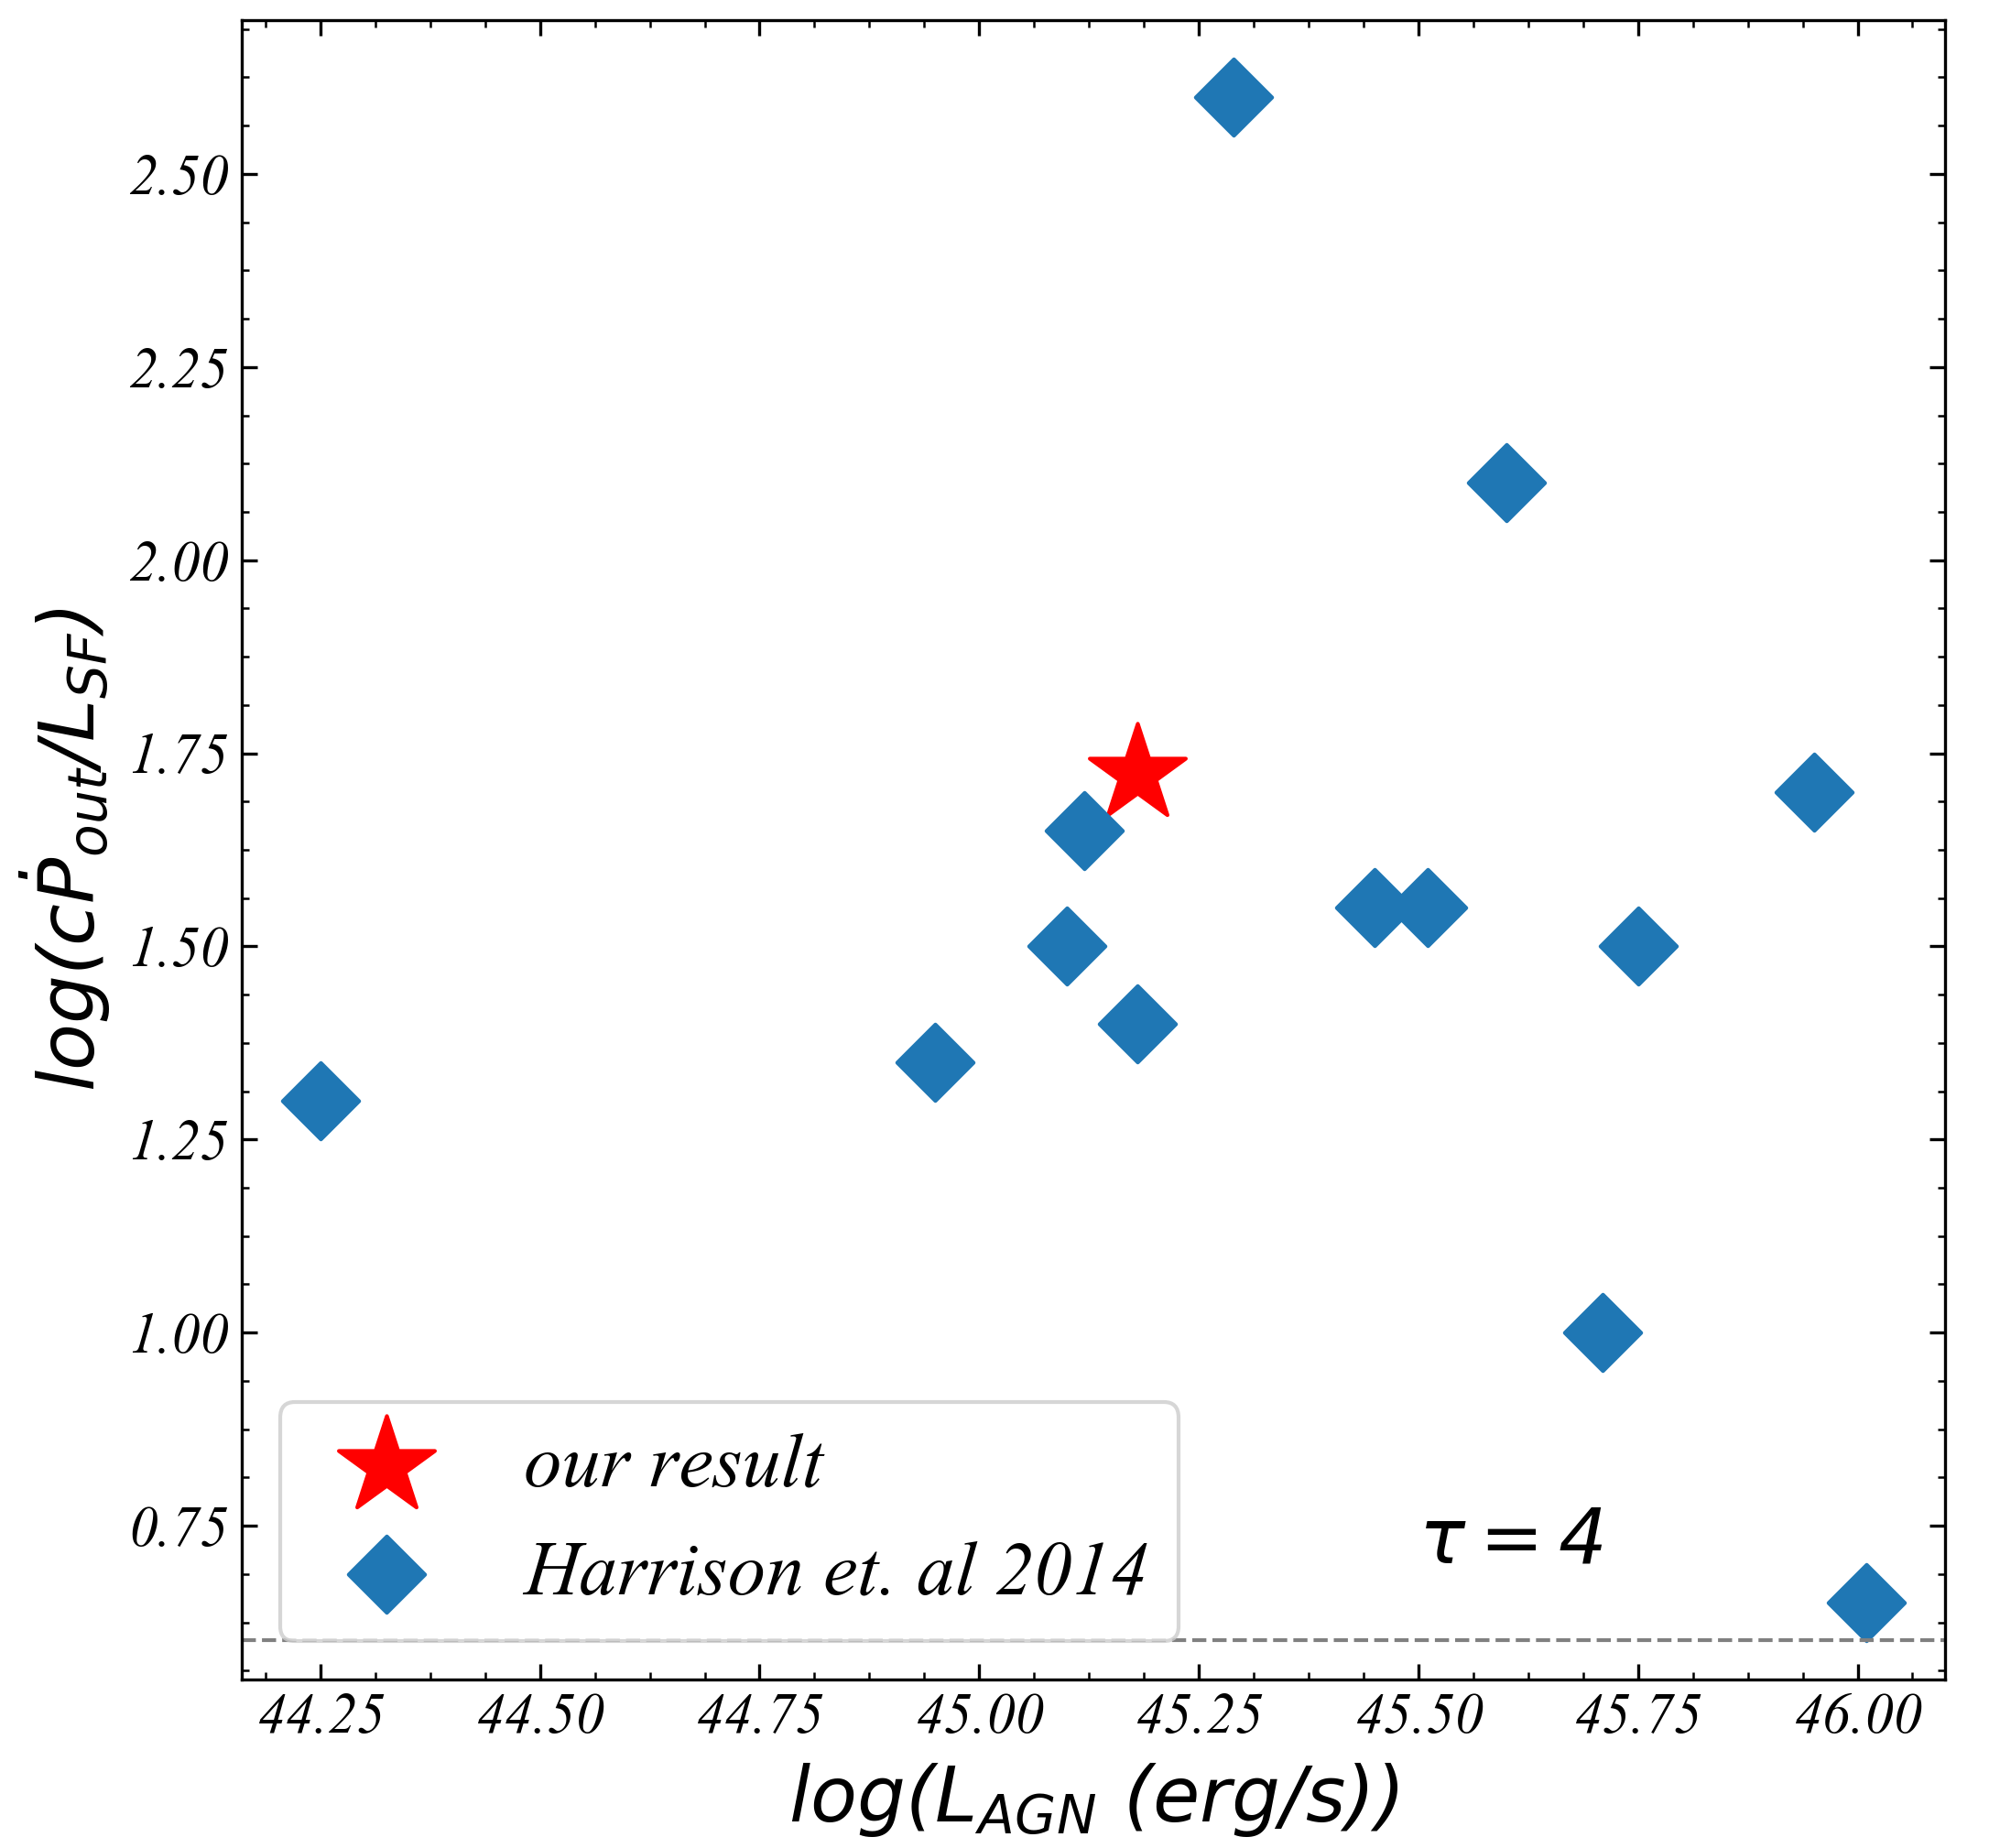
\includegraphics[width=0.5\textwidth]{figs/P_outSF_vs_L_AGN}}
		\subfloat{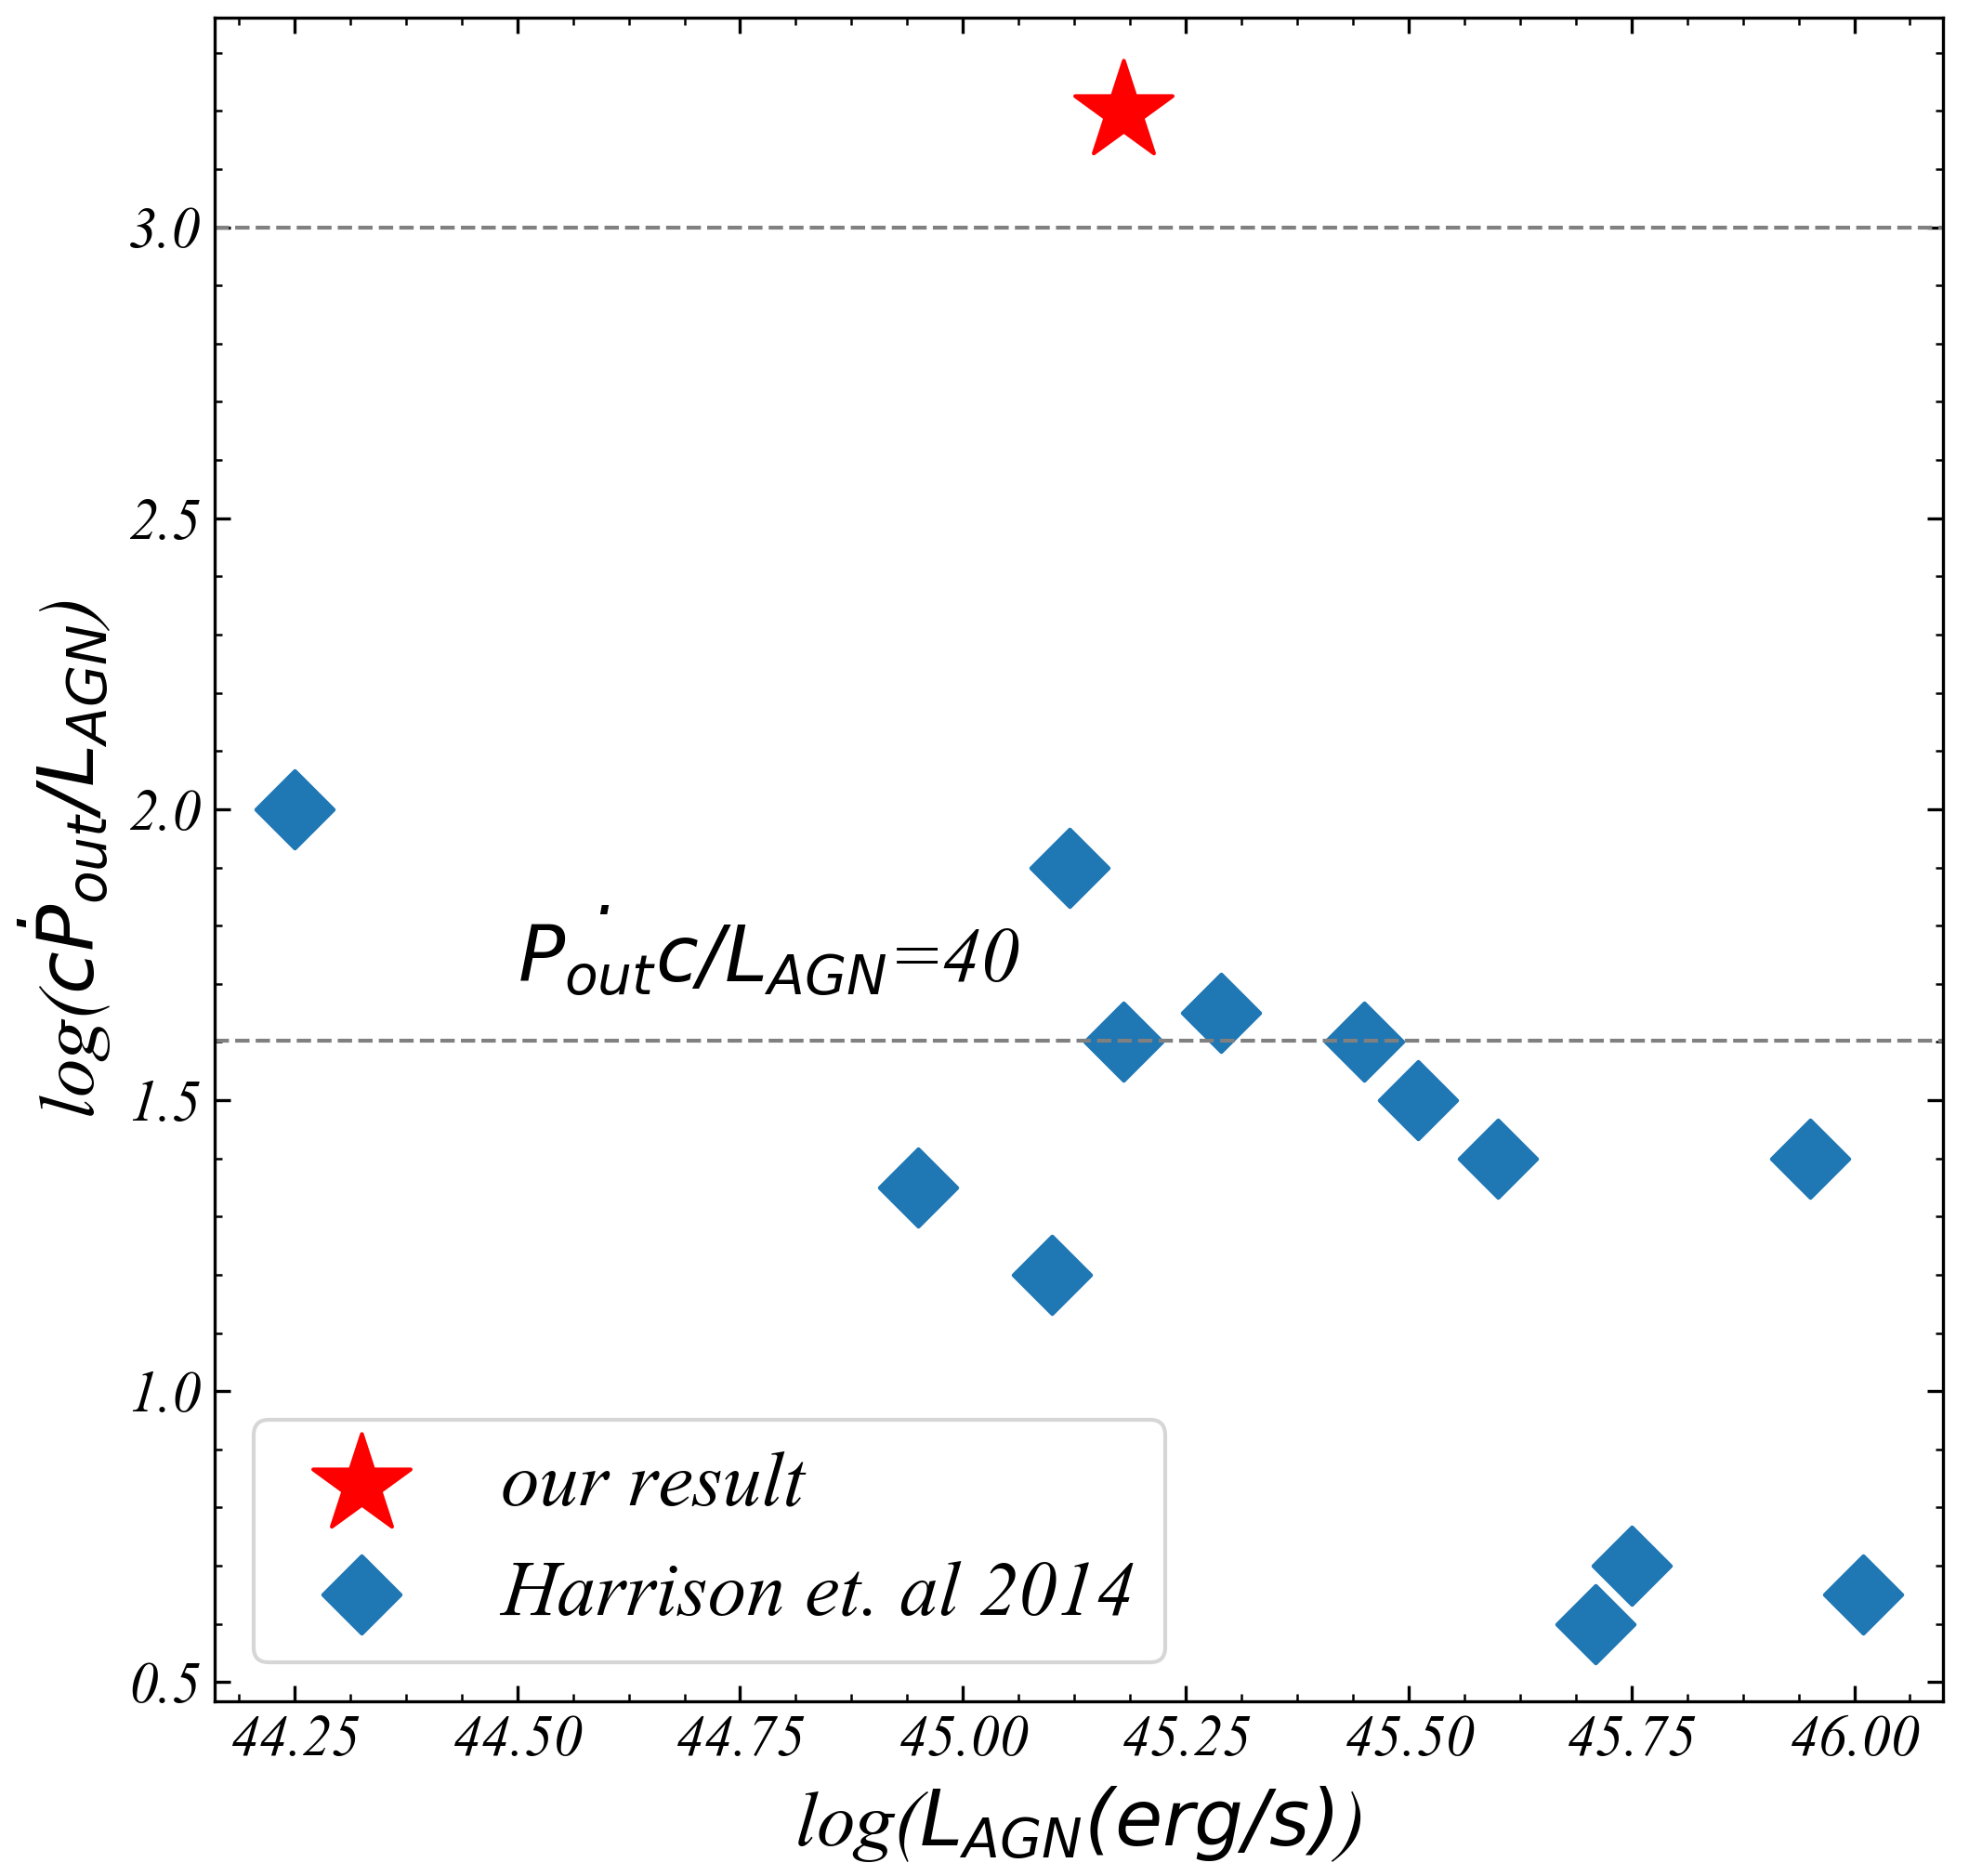
\includegraphics[width=0.5\textwidth]{figs/P_outAGN_vs_L_AGN}}
		\label{coupeffic}
		\caption{Left: momentum rates of the outflows($\dot{P_{out}}$ normalized to the star formation luminosity $L_{SF}/c$ versus AGN luminosity. The dashed lines represent the required optical depths if the outflows are driven by radiation pressure from star formation. Right: momentum rate of outflows normalized to AGN luminosity($L_{AGN}/c$) versus AGN luminosity. Based on our assumptions, the outflows are unlikely to be purely radiatively driven, the ratio is also to high for theoretical predictions of energy-driven outflows launched by AGN accretion-disc wind.}
	\end{figure*}
\end{document}